\subsection{Using a Library}

The code to use a library class looks just like any other class:
\begin{lstlisting}[language=Java]
package org.familysearch.viitanenm;

public class LibraryExample {

 public static void main(String[] args) {
   new LibraryExample().doIt();
 }

 private void doIt() {
  LibraryClass libraryClass = new LibraryClass();
  System.out.println(libraryClass.echo("Hello Library!"));
 }
}
\end{lstlisting}

In order to use a library we need to somehow tell our project where it is. We cannot just simply use a library class in another project or directory, even if the package name is the same.

\begin{figure}[H]\centering
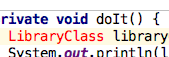
\includegraphics{images/library-error}
\caption{Library class not found}
\label{fig:libraryerror}
\end{figure}

We see that the LibraryClass is not found (in red), even if the class using it is in the same package. 

First we copy the library into our project. It really doesn't need to be in our project's directory structure, but it makes it easier to manage.

\begin{lstlisting}[language=Java]
.
+-- lib
|   +-- EchoLibrary.jar
+-- src
    +-- org
        +-- familysearch
            +-- viitanenm
                +-- LibraryExample.java
\end{lstlisting}

We can access the library by telling the compiler where it is. We do it by adding the library in the class path. If we are using and IDE, we can add the library as a dependency. We go to the top of our source code package structure. If we want to compile from command line, we use the -cp switch:

\begin{lstlisting}[language=Java]
javac -cp ../lib/EchoLibrary.jar org/familysearch/viitanenm/LibraryExample.java 
\end{lstlisting}

When we run it, we need to speficy the class path for our class (LibraryExample) and the class path for the library:
\begin{lstlisting}[language=Java]
java -cp .:../lib/EchoLibrary.jar org.familysearch.viitanenm.LibraryExample
\end{lstlisting}

The output is:
\begin{lstlisting}[language=Java]
Hello Library!
\end{lstlisting}
